% Created by tikzDevice version 0.12.3.1 on 2022-05-11 18:37:41
% !TEX encoding = UTF-8 Unicode
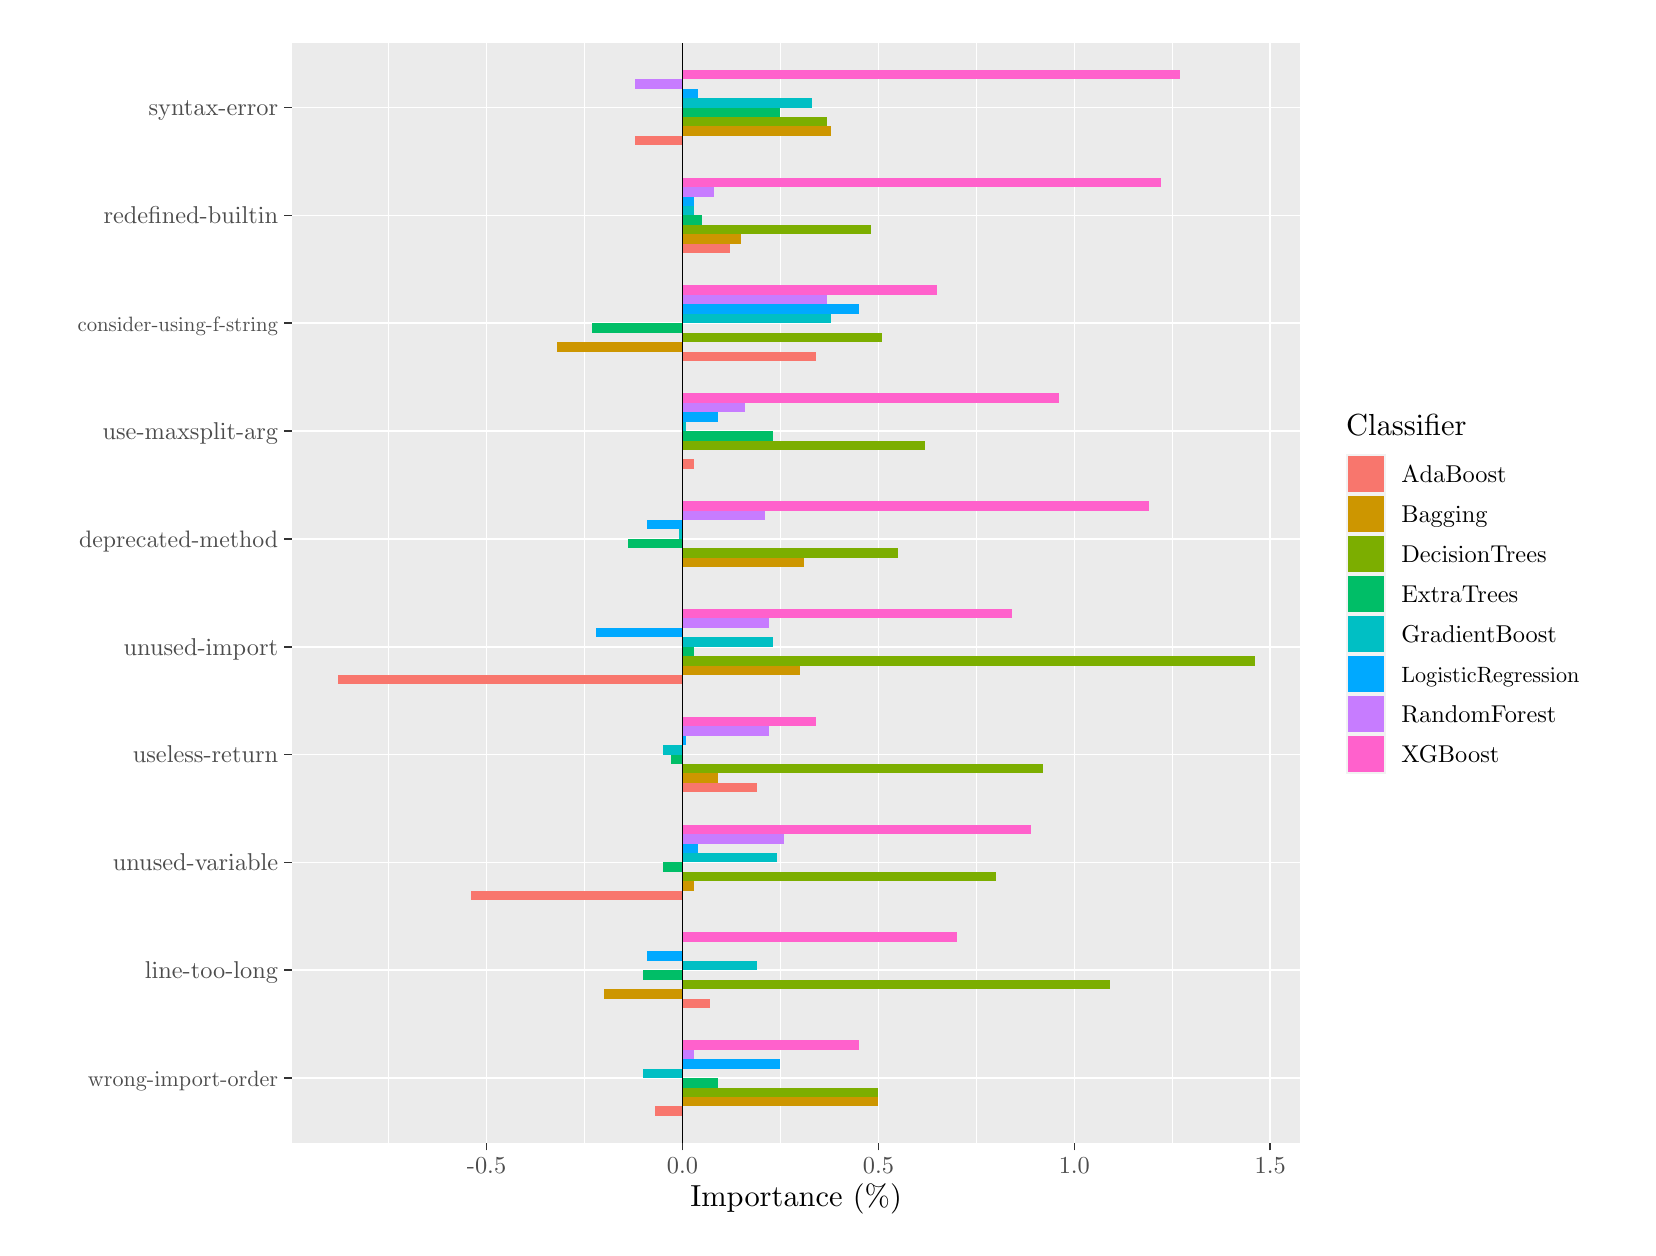
\begin{tikzpicture}[x=1pt,y=1pt]
\definecolor{fillColor}{RGB}{255,255,255}
\path[use as bounding box,fill=fillColor,fill opacity=0.00] (0,0) rectangle (578.16,433.62);
\begin{scope}
\path[clip] (  0.00,  0.00) rectangle (578.16,433.62);
\definecolor{drawColor}{RGB}{255,255,255}
\definecolor{fillColor}{RGB}{255,255,255}

\path[draw=drawColor,line width= 0.6pt,line join=round,line cap=round,fill=fillColor] (  0.00,  0.00) rectangle (578.16,433.62);
\end{scope}
\begin{scope}
\path[clip] ( 95.45, 30.69) rectangle (459.91,428.12);
\definecolor{fillColor}{gray}{0.92}

\path[fill=fillColor] ( 95.45, 30.69) rectangle (459.91,428.12);
\definecolor{drawColor}{RGB}{255,255,255}

\path[draw=drawColor,line width= 0.3pt,line join=round] (130.42, 30.69) --
	(130.42,428.12);

\path[draw=drawColor,line width= 0.3pt,line join=round] (201.22, 30.69) --
	(201.22,428.12);

\path[draw=drawColor,line width= 0.3pt,line join=round] (272.01, 30.69) --
	(272.01,428.12);

\path[draw=drawColor,line width= 0.3pt,line join=round] (342.81, 30.69) --
	(342.81,428.12);

\path[draw=drawColor,line width= 0.3pt,line join=round] (413.61, 30.69) --
	(413.61,428.12);

\path[draw=drawColor,line width= 0.6pt,line join=round] ( 95.45, 54.06) --
	(459.91, 54.06);

\path[draw=drawColor,line width= 0.6pt,line join=round] ( 95.45, 93.03) --
	(459.91, 93.03);

\path[draw=drawColor,line width= 0.6pt,line join=round] ( 95.45,131.99) --
	(459.91,131.99);

\path[draw=drawColor,line width= 0.6pt,line join=round] ( 95.45,170.96) --
	(459.91,170.96);

\path[draw=drawColor,line width= 0.6pt,line join=round] ( 95.45,209.92) --
	(459.91,209.92);

\path[draw=drawColor,line width= 0.6pt,line join=round] ( 95.45,248.88) --
	(459.91,248.88);

\path[draw=drawColor,line width= 0.6pt,line join=round] ( 95.45,287.85) --
	(459.91,287.85);

\path[draw=drawColor,line width= 0.6pt,line join=round] ( 95.45,326.81) --
	(459.91,326.81);

\path[draw=drawColor,line width= 0.6pt,line join=round] ( 95.45,365.78) --
	(459.91,365.78);

\path[draw=drawColor,line width= 0.6pt,line join=round] ( 95.45,404.74) --
	(459.91,404.74);

\path[draw=drawColor,line width= 0.6pt,line join=round] (165.82, 30.69) --
	(165.82,428.12);

\path[draw=drawColor,line width= 0.6pt,line join=round] (236.62, 30.69) --
	(236.62,428.12);

\path[draw=drawColor,line width= 0.6pt,line join=round] (307.41, 30.69) --
	(307.41,428.12);

\path[draw=drawColor,line width= 0.6pt,line join=round] (378.21, 30.69) --
	(378.21,428.12);

\path[draw=drawColor,line width= 0.6pt,line join=round] (449.00, 30.69) --
	(449.00,428.12);
\definecolor{fillColor}{RGB}{248,118,109}

\path[fill=fillColor] (219.62,391.10) rectangle (236.62,394.51);

\path[fill=fillColor] (236.62,352.14) rectangle (253.61,355.55);

\path[fill=fillColor] (236.62,313.18) rectangle (284.76,316.59);

\path[fill=fillColor] (236.62,274.21) rectangle (240.86,277.62);

\path[fill=fillColor] (236.62,235.25) rectangle (236.62,238.66);

\path[fill=fillColor] (112.01,196.28) rectangle (236.62,199.69);

\path[fill=fillColor] (236.62,157.32) rectangle (263.52,160.73);

\path[fill=fillColor] (160.16,118.36) rectangle (236.62,121.76);

\path[fill=fillColor] (236.62, 79.39) rectangle (246.53, 82.80);

\path[fill=fillColor] (226.70, 40.43) rectangle (236.62, 43.84);
\definecolor{fillColor}{RGB}{205,150,0}

\path[fill=fillColor] (236.62,394.51) rectangle (290.42,397.92);

\path[fill=fillColor] (236.62,355.55) rectangle (257.85,358.96);

\path[fill=fillColor] (191.31,316.59) rectangle (236.62,319.99);

\path[fill=fillColor] (236.62,277.62) rectangle (236.62,281.03);

\path[fill=fillColor] (236.62,238.66) rectangle (280.51,242.07);

\path[fill=fillColor] (236.62,199.69) rectangle (279.09,203.10);

\path[fill=fillColor] (236.62,160.73) rectangle (249.36,164.14);

\path[fill=fillColor] (236.62,121.76) rectangle (240.86,125.17);

\path[fill=fillColor] (208.30, 82.80) rectangle (236.62, 86.21);

\path[fill=fillColor] (236.62, 43.84) rectangle (307.41, 47.25);
\definecolor{fillColor}{RGB}{124,174,0}

\path[fill=fillColor] (236.62,397.92) rectangle (289.00,401.33);

\path[fill=fillColor] (236.62,358.96) rectangle (304.58,362.37);

\path[fill=fillColor] (236.62,319.99) rectangle (308.83,323.40);

\path[fill=fillColor] (236.62,281.03) rectangle (324.40,284.44);

\path[fill=fillColor] (236.62,242.07) rectangle (314.49,245.48);

\path[fill=fillColor] (236.62,203.10) rectangle (443.34,206.51);

\path[fill=fillColor] (236.62,164.14) rectangle (366.88,167.55);

\path[fill=fillColor] (236.62,125.17) rectangle (349.89,128.58);

\path[fill=fillColor] (236.62, 86.21) rectangle (390.95, 89.62);

\path[fill=fillColor] (236.62, 47.25) rectangle (307.41, 50.65);
\definecolor{fillColor}{RGB}{0,190,103}

\path[fill=fillColor] (236.62,401.33) rectangle (272.01,404.74);

\path[fill=fillColor] (236.62,362.37) rectangle (243.70,365.78);

\path[fill=fillColor] (204.05,323.40) rectangle (236.62,326.81);

\path[fill=fillColor] (236.62,284.44) rectangle (269.18,287.85);

\path[fill=fillColor] (216.79,245.48) rectangle (236.62,248.88);

\path[fill=fillColor] (236.62,206.51) rectangle (240.86,209.92);

\path[fill=fillColor] (232.37,167.55) rectangle (236.62,170.96);

\path[fill=fillColor] (229.54,128.58) rectangle (236.62,131.99);

\path[fill=fillColor] (222.46, 89.62) rectangle (236.62, 93.03);

\path[fill=fillColor] (236.62, 50.65) rectangle (249.36, 54.06);
\definecolor{fillColor}{RGB}{0,191,196}

\path[fill=fillColor] (236.62,404.74) rectangle (283.34,408.15);

\path[fill=fillColor] (236.62,365.78) rectangle (240.86,369.19);

\path[fill=fillColor] (236.62,326.81) rectangle (290.42,330.22);

\path[fill=fillColor] (236.62,287.85) rectangle (238.03,291.26);

\path[fill=fillColor] (235.20,248.88) rectangle (236.62,252.29);

\path[fill=fillColor] (236.62,209.92) rectangle (269.18,213.33);

\path[fill=fillColor] (229.54,170.96) rectangle (236.62,174.37);

\path[fill=fillColor] (236.62,131.99) rectangle (270.60,135.40);

\path[fill=fillColor] (236.62, 93.03) rectangle (263.52, 96.44);

\path[fill=fillColor] (222.46, 54.06) rectangle (236.62, 57.47);
\definecolor{fillColor}{RGB}{0,169,255}

\path[fill=fillColor] (236.62,408.15) rectangle (242.28,411.56);

\path[fill=fillColor] (236.62,369.19) rectangle (240.86,372.60);

\path[fill=fillColor] (236.62,330.22) rectangle (300.33,333.63);

\path[fill=fillColor] (236.62,291.26) rectangle (249.36,294.67);

\path[fill=fillColor] (223.87,252.29) rectangle (236.62,255.70);

\path[fill=fillColor] (205.47,213.33) rectangle (236.62,216.74);

\path[fill=fillColor] (236.62,174.37) rectangle (238.03,177.78);

\path[fill=fillColor] (236.62,135.40) rectangle (242.28,138.81);

\path[fill=fillColor] (223.87, 96.44) rectangle (236.62, 99.85);

\path[fill=fillColor] (236.62, 57.47) rectangle (272.01, 60.88);
\definecolor{fillColor}{RGB}{199,124,255}

\path[fill=fillColor] (219.62,411.56) rectangle (236.62,414.97);

\path[fill=fillColor] (236.62,372.60) rectangle (247.94,376.01);

\path[fill=fillColor] (236.62,333.63) rectangle (289.00,337.04);

\path[fill=fillColor] (236.62,294.67) rectangle (259.27,298.08);

\path[fill=fillColor] (236.62,255.70) rectangle (266.35,259.11);

\path[fill=fillColor] (236.62,216.74) rectangle (267.77,220.15);

\path[fill=fillColor] (236.62,177.78) rectangle (267.77,181.18);

\path[fill=fillColor] (236.62,138.81) rectangle (273.43,142.22);

\path[fill=fillColor] (236.62, 99.85) rectangle (236.62,103.26);

\path[fill=fillColor] (236.62, 60.88) rectangle (240.86, 64.29);
\definecolor{fillColor}{RGB}{255,97,204}

\path[fill=fillColor] (236.62,414.97) rectangle (416.44,418.38);

\path[fill=fillColor] (236.62,376.01) rectangle (409.36,379.41);

\path[fill=fillColor] (236.62,337.04) rectangle (328.65,340.45);

\path[fill=fillColor] (236.62,298.08) rectangle (372.54,301.49);

\path[fill=fillColor] (236.62,259.11) rectangle (405.11,262.52);

\path[fill=fillColor] (236.62,220.15) rectangle (355.55,223.56);

\path[fill=fillColor] (236.62,181.18) rectangle (284.76,184.59);

\path[fill=fillColor] (236.62,142.22) rectangle (362.63,145.63);

\path[fill=fillColor] (236.62,103.26) rectangle (335.73,106.67);

\path[fill=fillColor] (236.62, 64.29) rectangle (300.33, 67.70);
\definecolor{drawColor}{RGB}{0,0,0}

\path[draw=drawColor,line width= 0.6pt,line join=round] (236.62, 30.69) -- (236.62,428.12);
\end{scope}
\begin{scope}
\path[clip] (  0.00,  0.00) rectangle (578.16,433.62);
\definecolor{drawColor}{gray}{0.30}

\node[text=drawColor,anchor=base east,inner sep=0pt, outer sep=0pt, scale=  0.80] at ( 90.50, 51.03) {wrong-import-order};

\node[text=drawColor,anchor=base east,inner sep=0pt, outer sep=0pt, scale=  0.88] at ( 90.50, 90.00) {line-too-long};

\node[text=drawColor,anchor=base east,inner sep=0pt, outer sep=0pt, scale=  0.88] at ( 90.50,128.96) {unused-variable};

\node[text=drawColor,anchor=base east,inner sep=0pt, outer sep=0pt, scale=  0.88] at ( 90.50,167.93) {useless-return};

\node[text=drawColor,anchor=base east,inner sep=0pt, outer sep=0pt, scale=  0.88] at ( 90.50,206.89) {unused-import};

\node[text=drawColor,anchor=base east,inner sep=0pt, outer sep=0pt, scale=  0.86] at ( 90.50,245.85) {deprecated-method};

\node[text=drawColor,anchor=base east,inner sep=0pt, outer sep=0pt, scale=  0.88] at ( 90.50,284.82) {use-maxsplit-arg};

\node[text=drawColor,anchor=base east,inner sep=0pt, outer sep=0pt, scale=  0.75] at ( 90.50,323.78) {consider-using-f-string};

\node[text=drawColor,anchor=base east,inner sep=0pt, outer sep=0pt, scale=  0.88] at ( 90.50,362.75) {redefined-builtin};

\node[text=drawColor,anchor=base east,inner sep=0pt, outer sep=0pt, scale=  0.88] at ( 90.50,401.71) {syntax-error};
\end{scope}
\begin{scope}
\path[clip] (  0.00,  0.00) rectangle (578.16,433.62);
\definecolor{drawColor}{gray}{0.20}

\path[draw=drawColor,line width= 0.6pt,line join=round] ( 92.70, 54.06) --
	( 95.45, 54.06);

\path[draw=drawColor,line width= 0.6pt,line join=round] ( 92.70, 93.03) --
	( 95.45, 93.03);

\path[draw=drawColor,line width= 0.6pt,line join=round] ( 92.70,131.99) --
	( 95.45,131.99);

\path[draw=drawColor,line width= 0.6pt,line join=round] ( 92.70,170.96) --
	( 95.45,170.96);

\path[draw=drawColor,line width= 0.6pt,line join=round] ( 92.70,209.92) --
	( 95.45,209.92);

\path[draw=drawColor,line width= 0.6pt,line join=round] ( 92.70,248.88) --
	( 95.45,248.88);

\path[draw=drawColor,line width= 0.6pt,line join=round] ( 92.70,287.85) --
	( 95.45,287.85);

\path[draw=drawColor,line width= 0.6pt,line join=round] ( 92.70,326.81) --
	( 95.45,326.81);

\path[draw=drawColor,line width= 0.6pt,line join=round] ( 92.70,365.78) --
	( 95.45,365.78);

\path[draw=drawColor,line width= 0.6pt,line join=round] ( 92.70,404.74) --
	( 95.45,404.74);
\end{scope}
\begin{scope}
\path[clip] (  0.00,  0.00) rectangle (578.16,433.62);
\definecolor{drawColor}{gray}{0.20}

\path[draw=drawColor,line width= 0.6pt,line join=round] (165.82, 27.94) --
	(165.82, 30.69);

\path[draw=drawColor,line width= 0.6pt,line join=round] (236.62, 27.94) --
	(236.62, 30.69);

\path[draw=drawColor,line width= 0.6pt,line join=round] (307.41, 27.94) --
	(307.41, 30.69);

\path[draw=drawColor,line width= 0.6pt,line join=round] (378.21, 27.94) --
	(378.21, 30.69);

\path[draw=drawColor,line width= 0.6pt,line join=round] (449.00, 27.94) --
	(449.00, 30.69);
\end{scope}
\begin{scope}
\path[clip] (  0.00,  0.00) rectangle (578.16,433.62);
\definecolor{drawColor}{gray}{0.30}

\node[text=drawColor,anchor=base,inner sep=0pt, outer sep=0pt, scale=  0.88] at (165.82, 19.68) {-0.5};

\node[text=drawColor,anchor=base,inner sep=0pt, outer sep=0pt, scale=  0.88] at (236.62, 19.68) {0.0};

\node[text=drawColor,anchor=base,inner sep=0pt, outer sep=0pt, scale=  0.88] at (307.41, 19.68) {0.5};

\node[text=drawColor,anchor=base,inner sep=0pt, outer sep=0pt, scale=  0.88] at (378.21, 19.68) {1.0};

\node[text=drawColor,anchor=base,inner sep=0pt, outer sep=0pt, scale=  0.88] at (449.00, 19.68) {1.5};
\end{scope}
\begin{scope}
\path[clip] (  0.00,  0.00) rectangle (578.16,433.62);
\definecolor{drawColor}{RGB}{0,0,0}

\node[text=drawColor,anchor=base,inner sep=0pt, outer sep=0pt, scale=  1.10] at (277.68,  7.64) {Importance (\%)};
\end{scope}
\begin{scope}
\path[clip] (  0.00,  0.00) rectangle (578.16,433.62);
\definecolor{fillColor}{RGB}{255,255,255}

\path[fill=fillColor] (470.91,158.48) rectangle (572.66,300.33);
\end{scope}
\begin{scope}
\path[clip] (  0.00,  0.00) rectangle (578.16,433.62);
\definecolor{drawColor}{RGB}{0,0,0}

\node[text=drawColor,anchor=base west,inner sep=0pt, outer sep=0pt, scale=  1.10] at (476.41,286.18) {Classifier};
\end{scope}
\begin{scope}
\path[clip] (  0.00,  0.00) rectangle (578.16,433.62);
\definecolor{fillColor}{gray}{0.95}

\path[fill=fillColor] (476.41,265.16) rectangle (490.86,279.61);
\end{scope}
\begin{scope}
\path[clip] (  0.00,  0.00) rectangle (578.16,433.62);
\definecolor{fillColor}{RGB}{248,118,109}

\path[fill=fillColor] (477.12,265.87) rectangle (490.15,278.90);
\end{scope}
\begin{scope}
\path[clip] (  0.00,  0.00) rectangle (578.16,433.62);
\definecolor{fillColor}{gray}{0.95}

\path[fill=fillColor] (476.41,250.70) rectangle (490.86,265.16);
\end{scope}
\begin{scope}
\path[clip] (  0.00,  0.00) rectangle (578.16,433.62);
\definecolor{fillColor}{RGB}{205,150,0}

\path[fill=fillColor] (477.12,251.42) rectangle (490.15,264.45);
\end{scope}
\begin{scope}
\path[clip] (  0.00,  0.00) rectangle (578.16,433.62);
\definecolor{fillColor}{gray}{0.95}

\path[fill=fillColor] (476.41,236.25) rectangle (490.86,250.70);
\end{scope}
\begin{scope}
\path[clip] (  0.00,  0.00) rectangle (578.16,433.62);
\definecolor{fillColor}{RGB}{124,174,0}

\path[fill=fillColor] (477.12,236.96) rectangle (490.15,249.99);
\end{scope}
\begin{scope}
\path[clip] (  0.00,  0.00) rectangle (578.16,433.62);
\definecolor{fillColor}{gray}{0.95}

\path[fill=fillColor] (476.41,221.80) rectangle (490.86,236.25);
\end{scope}
\begin{scope}
\path[clip] (  0.00,  0.00) rectangle (578.16,433.62);
\definecolor{fillColor}{RGB}{0,190,103}

\path[fill=fillColor] (477.12,222.51) rectangle (490.15,235.54);
\end{scope}
\begin{scope}
\path[clip] (  0.00,  0.00) rectangle (578.16,433.62);
\definecolor{fillColor}{gray}{0.95}

\path[fill=fillColor] (476.41,207.34) rectangle (490.86,221.80);
\end{scope}
\begin{scope}
\path[clip] (  0.00,  0.00) rectangle (578.16,433.62);
\definecolor{fillColor}{RGB}{0,191,196}

\path[fill=fillColor] (477.12,208.05) rectangle (490.15,221.08);
\end{scope}
\begin{scope}
\path[clip] (  0.00,  0.00) rectangle (578.16,433.62);
\definecolor{fillColor}{gray}{0.95}

\path[fill=fillColor] (476.41,192.89) rectangle (490.86,207.34);
\end{scope}
\begin{scope}
\path[clip] (  0.00,  0.00) rectangle (578.16,433.62);
\definecolor{fillColor}{RGB}{0,169,255}

\path[fill=fillColor] (477.12,193.60) rectangle (490.15,206.63);
\end{scope}
\begin{scope}
\path[clip] (  0.00,  0.00) rectangle (578.16,433.62);
\definecolor{fillColor}{gray}{0.95}

\path[fill=fillColor] (476.41,178.43) rectangle (490.86,192.89);
\end{scope}
\begin{scope}
\path[clip] (  0.00,  0.00) rectangle (578.16,433.62);
\definecolor{fillColor}{RGB}{199,124,255}

\path[fill=fillColor] (477.12,179.15) rectangle (490.15,192.18);
\end{scope}
\begin{scope}
\path[clip] (  0.00,  0.00) rectangle (578.16,433.62);
\definecolor{fillColor}{gray}{0.95}

\path[fill=fillColor] (476.41,163.98) rectangle (490.86,178.43);
\end{scope}
\begin{scope}
\path[clip] (  0.00,  0.00) rectangle (578.16,433.62);
\definecolor{fillColor}{RGB}{255,97,204}

\path[fill=fillColor] (477.12,164.69) rectangle (490.15,177.72);
\end{scope}
\begin{scope}
\path[clip] (  0.00,  0.00) rectangle (578.16,433.62);
\definecolor{drawColor}{RGB}{0,0,0}

\node[text=drawColor,anchor=base west,inner sep=0pt, outer sep=0pt, scale=  0.88] at (496.36,269.35) {AdaBoost};
\end{scope}
\begin{scope}
\path[clip] (  0.00,  0.00) rectangle (578.16,433.62);
\definecolor{drawColor}{RGB}{0,0,0}

\node[text=drawColor,anchor=base west,inner sep=0pt, outer sep=0pt, scale=  0.88] at (496.36,254.90) {Bagging};
\end{scope}
\begin{scope}
\path[clip] (  0.00,  0.00) rectangle (578.16,433.62);
\definecolor{drawColor}{RGB}{0,0,0}

\node[text=drawColor,anchor=base west,inner sep=0pt, outer sep=0pt, scale=  0.88] at (496.36,240.45) {DecisionTrees};
\end{scope}
\begin{scope}
\path[clip] (  0.00,  0.00) rectangle (578.16,433.62);
\definecolor{drawColor}{RGB}{0,0,0}

\node[text=drawColor,anchor=base west,inner sep=0pt, outer sep=0pt, scale=  0.88] at (496.36,225.99) {ExtraTrees};
\end{scope}
\begin{scope}
\path[clip] (  0.00,  0.00) rectangle (578.16,433.62);
\definecolor{drawColor}{RGB}{0,0,0}

\node[text=drawColor,anchor=base west,inner sep=0pt, outer sep=0pt, scale=  0.88] at (496.36,211.54) {GradientBoost};
\end{scope}
\begin{scope}
\path[clip] (  0.00,  0.00) rectangle (578.16,433.62);
\definecolor{drawColor}{RGB}{0,0,0}

\node[text=drawColor,anchor=base west,inner sep=0pt, outer sep=0pt, scale=  0.80] at (496.36,197.08) {LogisticRegression};
\end{scope}
\begin{scope}
\path[clip] (  0.00,  0.00) rectangle (578.16,433.62);
\definecolor{drawColor}{RGB}{0,0,0}

\node[text=drawColor,anchor=base west,inner sep=0pt, outer sep=0pt, scale=  0.88] at (496.36,182.63) {RandomForest};
\end{scope}
\begin{scope}
\path[clip] (  0.00,  0.00) rectangle (578.16,433.62);
\definecolor{drawColor}{RGB}{0,0,0}

\node[text=drawColor,anchor=base west,inner sep=0pt, outer sep=0pt, scale=  0.88] at (496.36,168.18) {XGBoost};
\end{scope}
\end{tikzpicture}
